% !TEX program = xelatex
% Supporting Information, built as a separate document.
\documentclass[11pt,a4paper]{article}
\usepackage[margin=22mm,top=24mm,bottom=26mm]{geometry}
\usepackage{iftex}
\ifxetex
  \usepackage[defaultsups]{newtxtext}
  \usepackage{newtxmath}
  \setsansfont{texgyreheros}[Extension=.otf,UprightFont=*-regular,BoldFont=*-bold,ItalicFont=*-italic,BoldItalicFont=*-bolditalic,Scale=0.90]
\else
  \usepackage[T1]{fontenc}
  \usepackage[utf8]{inputenc}
  \usepackage[defaultsups]{newtxtext}
  \usepackage{newtxmath}
  \usepackage[scaled=0.90]{helvet}
\fi
\emergencystretch=1.5em
\usepackage{microtype}
\usepackage{amsmath}
\usepackage{booktabs}
\usepackage{graphicx}
\usepackage{xcolor}
\usepackage{caption}
\usepackage{subcaption}
\usepackage{titlesec}
\usepackage{authblk}
\usepackage{url}
\usepackage[colorlinks=true,allcolors={blue!55!black}]{hyperref}
\graphicspath{{figures/}}
\captionsetup{font=small,labelfont={bf,sf},labelsep=period,justification=justified}
\titleformat{\section}{\sffamily\bfseries\large}{\thesection}{0.8em}{}
\titleformat{\subsection}{\sffamily\bfseries}{\thesubsection}{0.8em}{}
\setlength{\parskip}{0pt}
\renewcommand\Authfont{\normalsize}
\renewcommand\Affilfont{\small\itshape}
\renewcommand{\thetable}{S\arabic{table}}
\renewcommand{\thefigure}{S\arabic{figure}}
\newcommand{\studio}{MOSAICS Studio}
\newcommand{\kcal}{kcal/mol}
\urlstyle{same}

\title{\sffamily\bfseries\large Supporting Information\\[3pt]
\normalsize\mdseries \studio{}: all-atom natural-move Monte Carlo on modern
additive force fields in the browser}
\author[1]{Folorunsho Bright Omage}
\author[1]{Peter Minary}
\affil[1]{Department of Computer Science, University of Oxford, Oxford OX1 3QD, United Kingdom}
\date{8 September 2026}

\begin{document}
\maketitle
\section*{Supporting Information}
\setcounter{table}{0}
\renewcommand{\thetable}{S\arabic{table}}

This file collects the settings, counts and file-level detail a reader
needs in order to rerun a job or check a number, and nothing that carries an
argument in the main text. Every entry is read from a committed file, and the
file is named in each caption.

\subsection*{S1. MOSAICS single-point settings}

Table~\ref{tab:si-mosaics} lists the settings that turn a MOSAICS Monte
Carlo job into a single-point energy evaluation. The committed inputs are
\path{evidence/1efs/<ff>/mosaics/*.input} and
\path{evidence/protein/<ff>/mosaics/*.input}.

\begin{table}[h]
\centering
\footnotesize
\caption{The MOSAICS input settings common to every run reported in this work,
in the engine's own syntax, with the two that differ between the two test
systems at the foot.}
\label{tab:si-mosaics}
\begin{tabular}{lll}
\toprule
Setting & Value & Effect \\
\midrule
\texttt{\textbackslash prop\_tors\_sig}   & \texttt{0.0} & torsional proposal width \\
\texttt{\textbackslash prop\_trans\_sig}  & \texttt{0.0} & translational proposal width \\
\texttt{\textbackslash prop\_rot\_sig}    & \texttt{0.0} & rotational proposal width \\
\texttt{\textbackslash total\_step\_mc}   & \texttt{1}   & one Monte Carlo step \\
\texttt{\textbackslash local\_step\_md}   & \texttt{1}   & one inner step per move \\
\texttt{\textbackslash statistics\_freq}  & \texttt{1}   & report every step \\
\texttt{\textbackslash energy\_report}    & \texttt{2}   & print each term and each part of each term \\
\texttt{\textbackslash implicit\_solvent} & \texttt{off} & vacuum \\
\texttt{\textbackslash ddd}               & \texttt{off} & no distance-dependent dielectric \\
\texttt{\textbackslash neutralize}        & \texttt{off} & net charge kept \\
\texttt{\textbackslash inter\_list}       & \texttt{none}& no neighbour list; all non-excluded pairs \\
\texttt{\textbackslash rinter\_switch\_length}  & \texttt{0}    & no switching function \\
\texttt{\textbackslash rinter\_exclude\_length} & \texttt{1000} & no interaction excluded by distance \\
\texttt{\textbackslash write\_energy\_unit}     & \texttt{kcal} & output in kcal/mol \\
\texttt{\textbackslash temperature}             & \texttt{300}  & read, but nothing is propagated \\
\midrule
\texttt{\textbackslash prop\_type}    & \texttt{tors} (1efs), \texttt{cart} (peptide) & proposal coordinate \\
\texttt{\textbackslash time\_step\_md}& \texttt{0.4} (1efs), \texttt{0.0} (peptide)   & zero is required in Cartesian mode \\
\bottomrule
\end{tabular}
\end{table}

\subsection*{S2. Deck sizes}

Table~\ref{tab:si-decks} gives the entry counts the engine prints as it
reads each deck, taken from the \texttt{Database reading done} lines of
\texttt{mosaics\_sp.out} in each run directory. The counts are properties
of the deck and not of the test system: they say how many parameter rows were
available, not how many were used, and the engine does not report how many rows
a given structure selects.

\begin{table}[h]
\centering
\footnotesize
\caption{Entries read from each file of each deck, from the
\texttt{mosaics\_sp.out} of the run named in the last column. The
\texttt{.onfo} and \texttt{.vdw} files carry the same number of rows by
construction.}
\label{tab:si-decks}
\begin{tabular}{lrrrrrl}
\toprule
Deck & \texttt{.bond} & \texttt{.bend} & \texttt{.tors\_and\_impr} & \texttt{.onfo} & \texttt{.vdw} & Run \\
\midrule
\texttt{db\_ff14sb}    &  90 & 258 &  526 &  595 &  595 & \texttt{protein/ff14sb} \\
\texttt{db\_ff19sb}    & 102 & 329 &  690 &  666 &  666 & \texttt{protein/ff19sb} \\
\texttt{db\_bs0}       & 175 & 567 & 1060 & 2145 & 2145 & \texttt{1efs/bs0} \\
\texttt{db\_bsc1}      & 144 & 350 &  660 & 2211 & 2211 & \texttt{1efs/bsc1} \\
\texttt{db\_ol15\_ol3} & 145 & 371 &  487 & 1596 & 1596 & \texttt{1efs/ol15\_ol3} \\
\texttt{db\_ol21\_ol3} & 150 & 388 &  557 & 1596 & 1596 & \texttt{1efs/ol21\_ol3} \\
\bottomrule
\end{tabular}
\end{table}

The ff19SB deck carries a sixth file. On the peptide the engine reads 44
\texttt{.cmap} database entries, loads 16 maps at a grid of $N=24$ and
selects four of them, one per interior residue:
\path{evidence/protein/ff19sb/mosaics/mosaics_sp.out} line 147 reads
\texttt{cmap: 16 map(s) loaded (N=24), 4 backbone term(s)}. The CHARMM36
nucleic deck is counted differently, because it is generated rather than
converted row by row; its manifest,
\texttt{params/db\_charmm36\_na/manifest.tsv}, records 24 residues, 237
bonds, 562 bends, 1036 torsion entries and 15\,753 non-bonded pairs.

\subsection*{S3. Reference-engine control files}

Table~\ref{tab:si-controls} reproduces the three control files in full.
Each is committed at the path given in Table~1 of the main text. The GROMACS
cutoff is constructed per structure rather than chosen: for a largest
interatomic distance $d$, the cubic box edge is set to $2d+4$\,nm and the
cutoff to half of it, $d+2$\,nm, which puts every pair in the molecule
inside the cutoff with 2\,nm to spare and every periodic image outside it. That
gives $5.775263$\,nm on 1efs and $2.973662$\,nm on the peptide.
The run confirms the cutoff does nothing: \texttt{sp.log} reports
\texttt{Potential shift: LJ r\^{}-12: 0.000e+00 r\^{}-6: 0.000e+00,
Coulomb -0e+00}.

\begin{table}[h]
\centering
\footnotesize
\caption{The complete control settings for the three reference engines.
\texttt{rlist}, \texttt{rcoulomb} and \texttt{rvdw} are set equal to each other
and per structure, as described above.}
\label{tab:si-controls}
\begin{tabular}{lll}
\toprule
Engine & Setting & Value \\
\midrule
sander  & \texttt{imin}   & \texttt{1} \\
        & \texttt{maxcyc} & \texttt{0} \\
        & \texttt{ntb}    & \texttt{0} \\
        & \texttt{cut}    & \texttt{999.0} \\
        & \texttt{ntpr}   & \texttt{1} \\
        & \texttt{dielc}  & \texttt{1.0} \\
\midrule
OpenMM  & \texttt{nonbondedMethod} & \texttt{NoCutoff} \\
        & \texttt{constraints}     & \texttt{None} \\
        & \texttt{rigidWater}      & \texttt{False} \\
        & \texttt{removeCMMotion}  & \texttt{False} \\
        & \texttt{implicitSolvent} & \texttt{None} \\
        & platform                 & Reference, double precision \\
\midrule
GROMACS & \texttt{integrator}     & \texttt{md} \\
        & \texttt{nsteps}         & \texttt{0} \\
        & \texttt{cutoff-scheme}  & \texttt{Verlet} \\
        & \texttt{verlet-buffer-tolerance} & \texttt{-1} \\
        & \texttt{coulombtype}    & \texttt{Cut-off} \\
        & \texttt{vdwtype}        & \texttt{Cut-off} \\
        & \texttt{coulomb-modifier} & \texttt{None} \\
        & \texttt{vdw-modifier}   & \texttt{None} \\
        & \texttt{epsilon-r}      & \texttt{1} \\
        & \texttt{epsilon-rf}     & \texttt{1} \\
        & \texttt{DispCorr}       & \texttt{no} \\
        & \texttt{constraints}    & \texttt{none} \\
\bottomrule
\end{tabular}
\end{table}

\subsection*{S4. The four 1efs \texttt{tleap} presets}

Table~\ref{tab:si-presets} sets the four committed \texttt{tleap}
inputs against each other. The files are
\path{evidence/1efs/<ff>/topology/build_<ff>.in}. Three things differ
between them: the parameter files loaded, an \texttt{addAtomTypes} block
that only the bsc1 preset carries, and the residue names used for the RNA strand.
The last two follow from the libraries. \texttt{parmBSC1.lib} uses the
carbon types C1, C2, CI and CE, which \texttt{oldff/leaprc.ff99} either
does not define or defines with a different hybridisation, so they have to be
declared before the library is loaded; the block is the one AmberTools ships in
its own \texttt{leaprc.DNA.bsc1}. The ff99 nucleic library names its RNA
units RU, RC, RU5 and RC3, while the OL3 RNA library names the same units U, C,
U5 and C3. The residues built are the same either way, which
\texttt{residue\_mapping.tsv} confirms residue by residue, every row
carrying \texttt{base\_match True}.

\begin{table}[h]
\centering
\footnotesize
\caption{The four 1efs \texttt{tleap} presets. All four build the same padded
30-residue system of 942 atoms and are then trimmed to 818 atoms in 26 residues
by removing the first and last residue of each strand.
\texttt{renamed\_atoms} is the field of that name in
\texttt{build\_metadata.json}.}
\label{tab:si-presets}
\begin{tabular}{llll}
\toprule
Preset & Parameter files loaded & RNA strand written as & \texttt{renamed\_atoms} \\
\midrule
OL21/OL3 & \texttt{leaprc.DNA.OL21}, \texttt{leaprc.RNA.OL3} & \texttt{U5 U \dots{} C C3} & 0 \\
OL15/OL3 & \texttt{leaprc.DNA.OL15}, \texttt{leaprc.RNA.OL3} & \texttt{U5 U \dots{} C C3} & 0 \\
parmbsc1 & \texttt{oldff/leaprc.ff99}, then & \texttt{RU5 RU \dots{} RC RC3} & 88 \\
         & \texttt{addAtomTypes} for C1, C2, CI, CE, then & & \\
         & \texttt{frcmod.parmbsc0}, \texttt{parmBSC1.lib}, \texttt{frcmod.parmbsc1} & & \\
parmbsc0 & \texttt{oldff/leaprc.ff99bsc0} & \texttt{RU5 RU \dots{} RC RC3} & 176 \\
\bottomrule
\end{tabular}
\end{table}

The \texttt{renamed\_atoms} field counts substitutions performed by
\texttt{rename\_atoms\_to\_modern} in
\path{tools/build_1efs_amber_reference.py}, which walks the built
structure and rewrites seven legacy AMBER atom names into their PDB~v3
equivalents: O1P and O2P to OP1 and OP2, H5$'$1 and H5$'$2 to H5$'$ and
H5$''$, H2$'$1 and H2$'$2 to H2$'$ and H2$''$, and HO$'$2 to HO2$'$. It changes
names only, and it runs after \texttt{tleap} has assigned every type and
charge, so it cannot alter an energy. The two counts follow from which library
supplied each strand. In bs0 both strands come from ff99bsc0 and carry the
legacy names throughout, giving $2\times28$ phosphate oxygens on the 28
residues that have a phosphate, $2\times30$ H5$'$ hydrogens, 30 on the
DNA H2$'$ pair and 30 on the RNA H2$'$/HO$'$2 pair, which is 176. In bsc1 the
DNA residues come from \texttt{parmBSC1.lib}, which already writes OP1,
OP2, H5$'$, H5$''$, H2$'$ and H2$''$, so only the ff99 RNA strand is rewritten:
28 phosphate oxygens on its 14 phosphates, 30 H5$'$ hydrogens, 15 H2$'$1 and 15
HO$'$2, which is 88. The OL libraries write the modern names on both strands and
need none.

\subsection*{S5. Reading a number out of the committed files}

Table~\ref{tab:si-commands} gives one command per engine, to be run from
the \texttt{evidence/} folder.

\begin{table}[h]
\centering
\footnotesize
\caption{Commands that print the committed energies. Paths are relative to
\texttt{evidence/}.}
\label{tab:si-commands}
\begin{tabular}{ll}
\toprule
Engine & Command \\
\midrule
sander  & \texttt{awk '/FINAL RESULTS/,0' */sander/*\_sander\_sp.out} \\
OpenMM  & \texttt{cat */openmm/openmm\_sp.out} \\
GROMACS & \texttt{tail -1 */gromacs/sp.xvg} \\
MOSAICS & \texttt{grep 'Initial .* energy' */mosaics/mosaics\_sp.out} \\
\bottomrule
\end{tabular}
\end{table}

\subsection*{S6. The CHARMM36 conversion route}

The full account is \texttt{evidence/charmm36.txt}. Four points of
detail sit behind the summary in the main text.

\emph{The release.} Two OpenMM force-field XML files of the CHARMM36
nucleic acid parameters were available, and only one of them can be used.
\texttt{charmm36.xml} cannot build a strand: its five nucleic templates
each declare a single external bond, on O3$'$ and not on P, and none of its 107
patches is a $5'$ patch, so it describes mononucleotides and OpenMM cannot
produce a reference energy from it. \texttt{charmm36\_2024.xml} declares
external bonds on both O3$'$ and P and ships the $5'$ patches 5TER, 5MET, 5PHO
and 5POM, and is the file used; it carries 100\,295 atom types against the 412
of \texttt{charmm36.xml}. It also generates its impropers when it loads
instead of declaring them in the file, so the deck is read out of the built
OpenMM \texttt{System} by
\texttt{tools/openmm\_system\_to\_mosaics.py} rather than out of the XML,
and the reference energies come from
\texttt{tools/charmm\_reference\_energy.py} on the same file.

\emph{Urey--Bradley.} The $1$--$3$ harmonic is written into the bond slot
of the \texttt{\~{}bend\_parm} record, which the engine already evaluates
as $\tfrac{1}{2}k(r_{13}-r_0)^2$. Of 810 unordered triples, 807 are
emitted and three are dropped and counted: the P--ON2--P entries and their P3
variants carry a negative force constant, which the deck reader rejects for the
whole file. They are pyrophosphate linkages and do not occur in a
phosphodiester backbone.

\emph{Harmonic impropers.} The 188 harmonic impropers are carried as
\texttt{\~{}torsion\_parm} records with
\texttt{\textbackslash pot\_type\{harm\}}, which the deck reader expands
into a truncated sixth-order Fourier series. That truncation is the only genuine
approximation in the conversion, and Table~\ref{tab:si-improper} gives its error
against the harmonic it replaces. Nucleobase impropers are stiff and stay inside
$20^{\circ}$ of equilibrium in the structures used here; the series is
not exercised further out by any run in this paper.

\begin{table}[h]
\centering
\footnotesize
\caption{Error of the truncated sixth-order Fourier expansion against the
harmonic improper it replaces, as a fraction of the harmonic energy at that
displacement from equilibrium.}
\label{tab:si-improper}
\begin{tabular}{lr}
\toprule
Displacement from equilibrium & Error \\
\midrule
$10^{\circ}$ & exact to four figures \\
$30^{\circ}$ & $-0.2$\,\% \\
$45^{\circ}$ & $-1.8$\,\% \\
$60^{\circ}$ & $-7.7$\,\% \\
\bottomrule
\end{tabular}
\end{table}

\emph{Generating the deck.} A CHARMM36 deck has to be generated from a
structure carrying every residue in every position it will be used in, so the
committed deck comes from 24 residues covering each of the four DNA and four RNA
bases as $5'$, internal and $3'$. MOSAICS builds a torsion for every bonded
one-four pair and stops if the deck has no row for it, whereas CHARMM simply
omits an unparameterised quadruplet, so the converter writes an explicit
zero-energy row in those cases: 197 of them on this deck.

\subsection*{S7. The 1efs coordinate edits}

Model 1 of PDB entry 1EFS was taken as deposited and edited in two ways:
six atoms were built, and four further operations rename or renumber what was
already there. Nothing else about the coordinates was touched -- the hydrogens
are the deposited NMR hydrogens, none was rebuilt, and no minimisation was
performed in this or any other force field. The pipeline is
\texttt{build\_1efs\_pipeline.sh} with the four scripts it calls.

The six built atoms are two $5'$ phosphate groups, P, OP1 and OP2, one on
chain A residue 1 and one on chain B residue 26. Both strands open on a $5'$
terminus without a phosphate, and the engine's bulk-residue templates expect
one. Each group was built by taking the neighbouring residue's phosphate and
applying the rigid transformation that maps that neighbour's C5$'$--O5$'$ frame
onto the terminal residue's, so the geometry of the added group is the deposited
geometry of its neighbour and no internal coordinate was invented.

The four further edits are: OP1 and OP2 renamed to O1P and O2P; the RNA
H2$'$ and HO2$'$ pair swapped to the MOSAICS convention; the $3'$ HO3$'$ dropped
on the two $3'$ residues; and chain B renumbered so that ascending residue
number runs $5'$ to $3'$.


\subsection*{S8. The page, Start and Run steps}

\begin{figure}[h]
\centering
\begin{subfigure}[t]{0.84\linewidth}
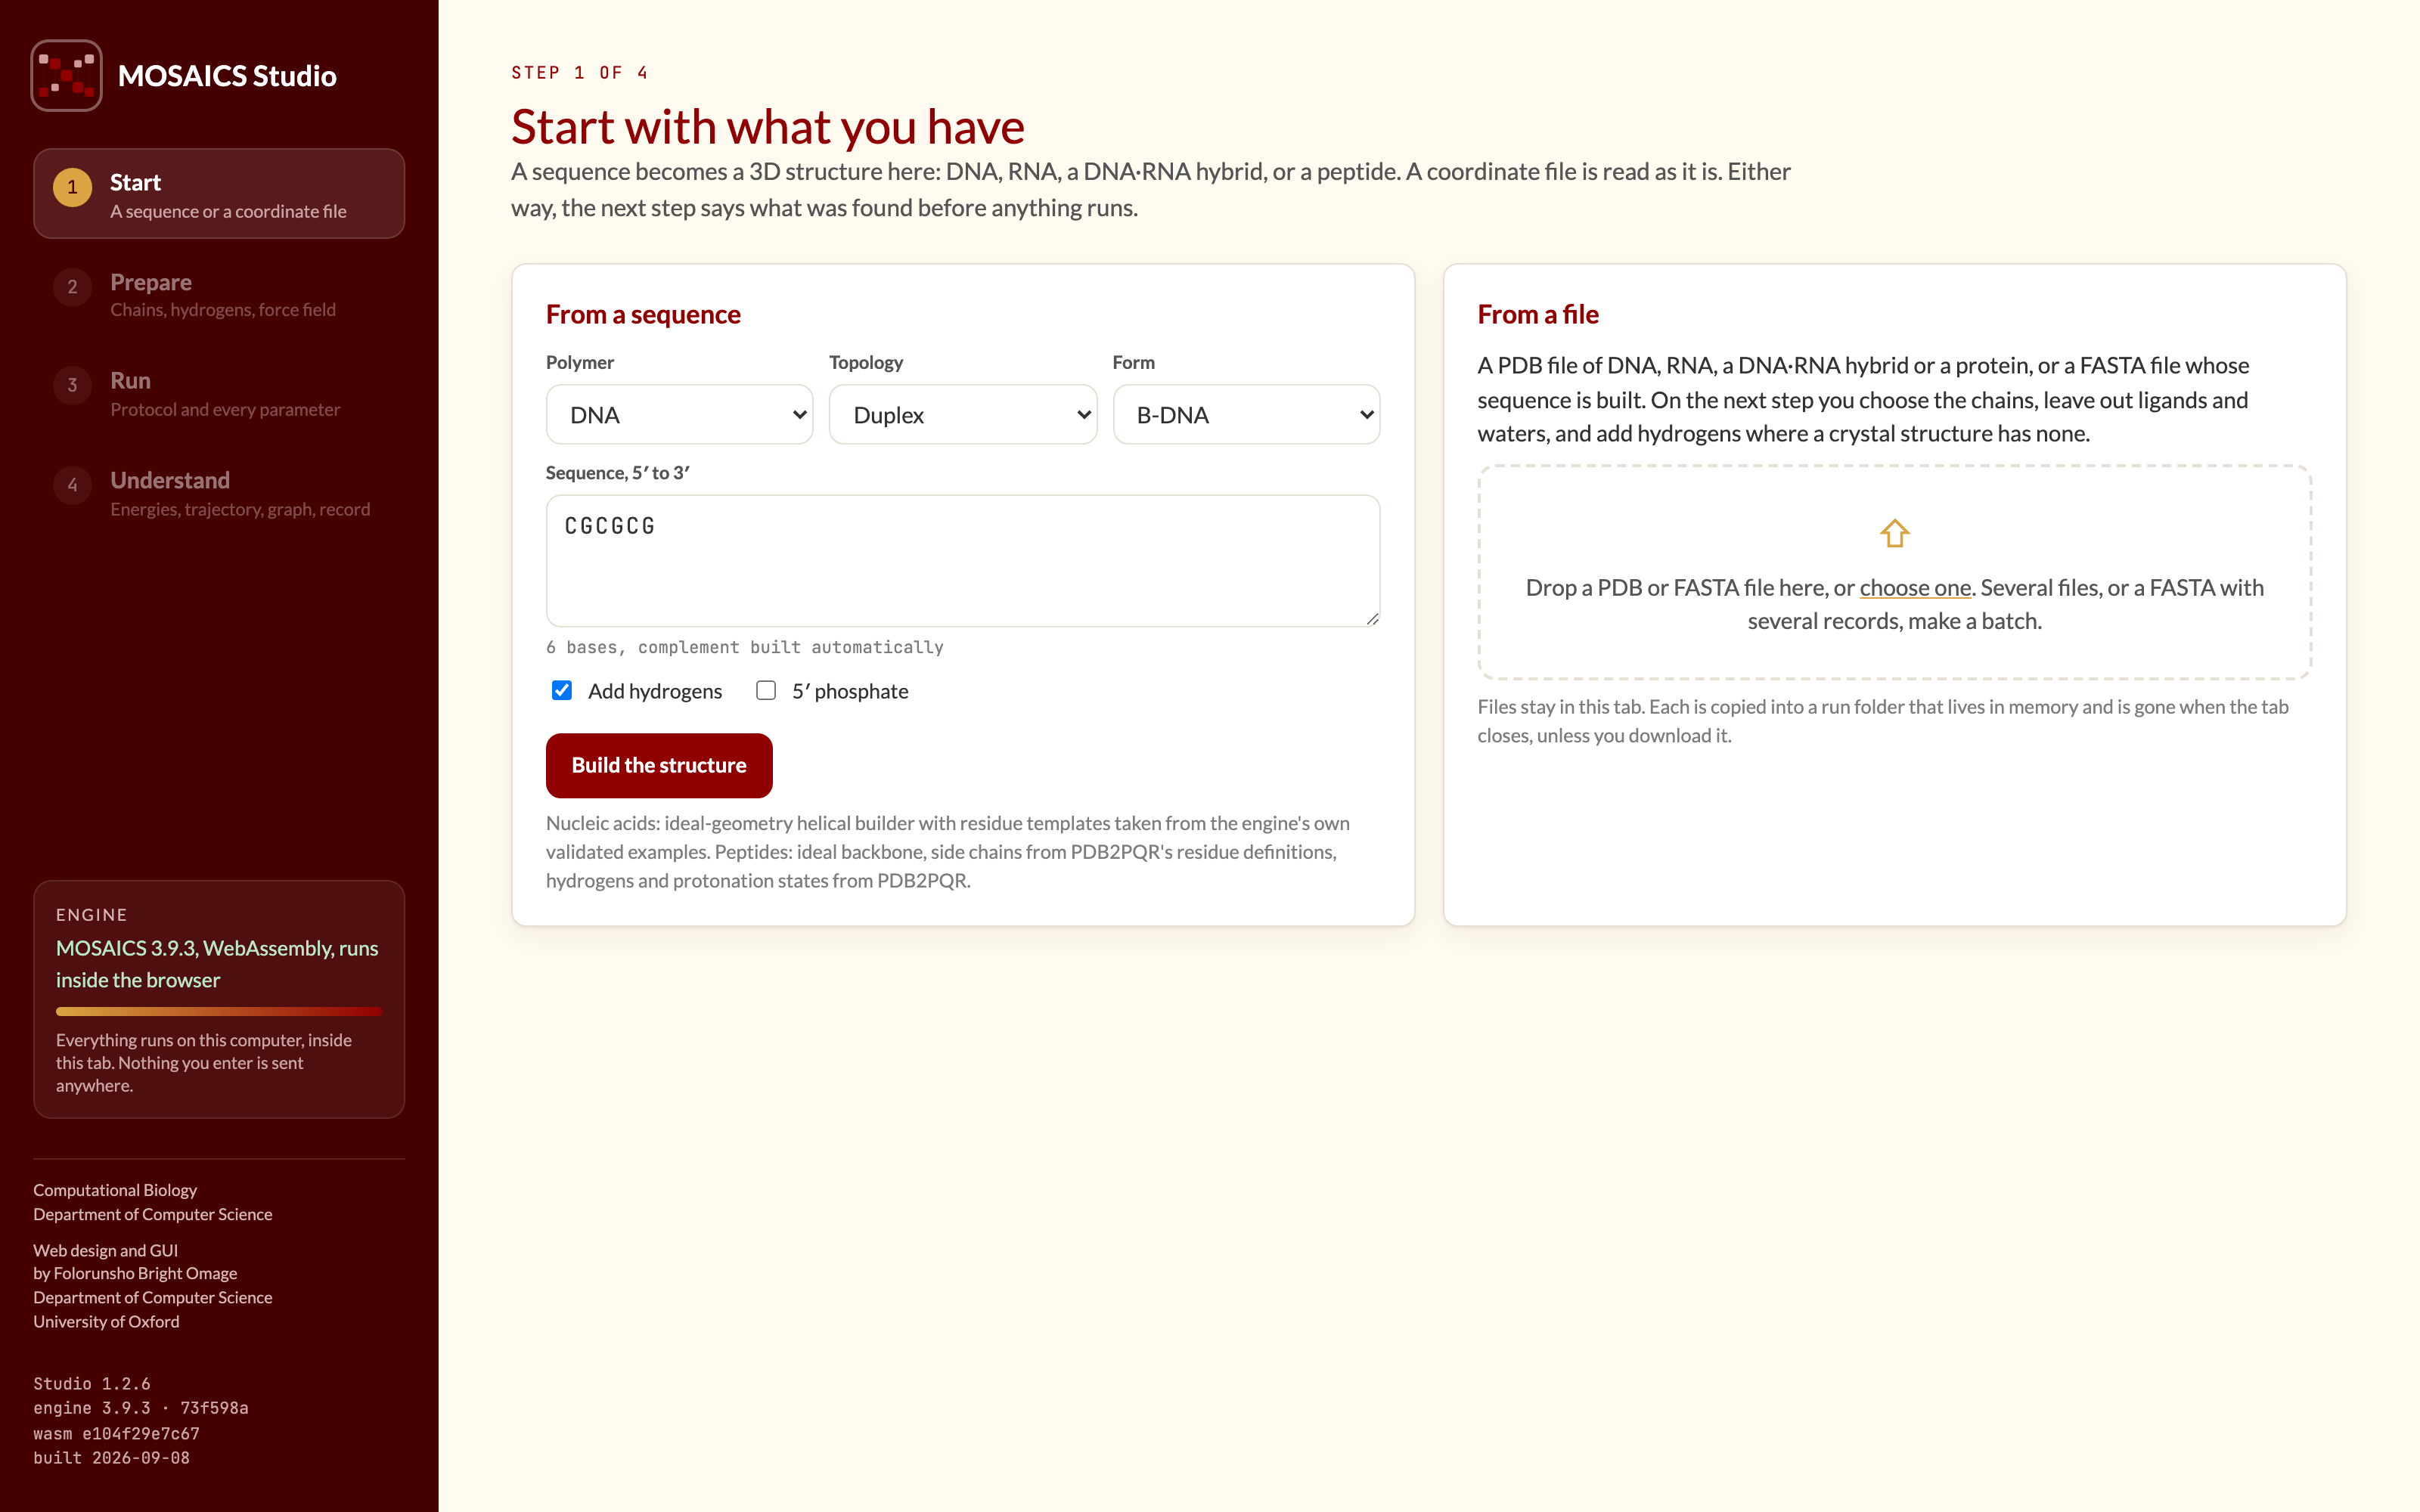
\includegraphics[width=\linewidth]{studio-start.png}
\caption{}
\end{subfigure}
\par\medskip
\begin{subfigure}[t]{0.84\linewidth}
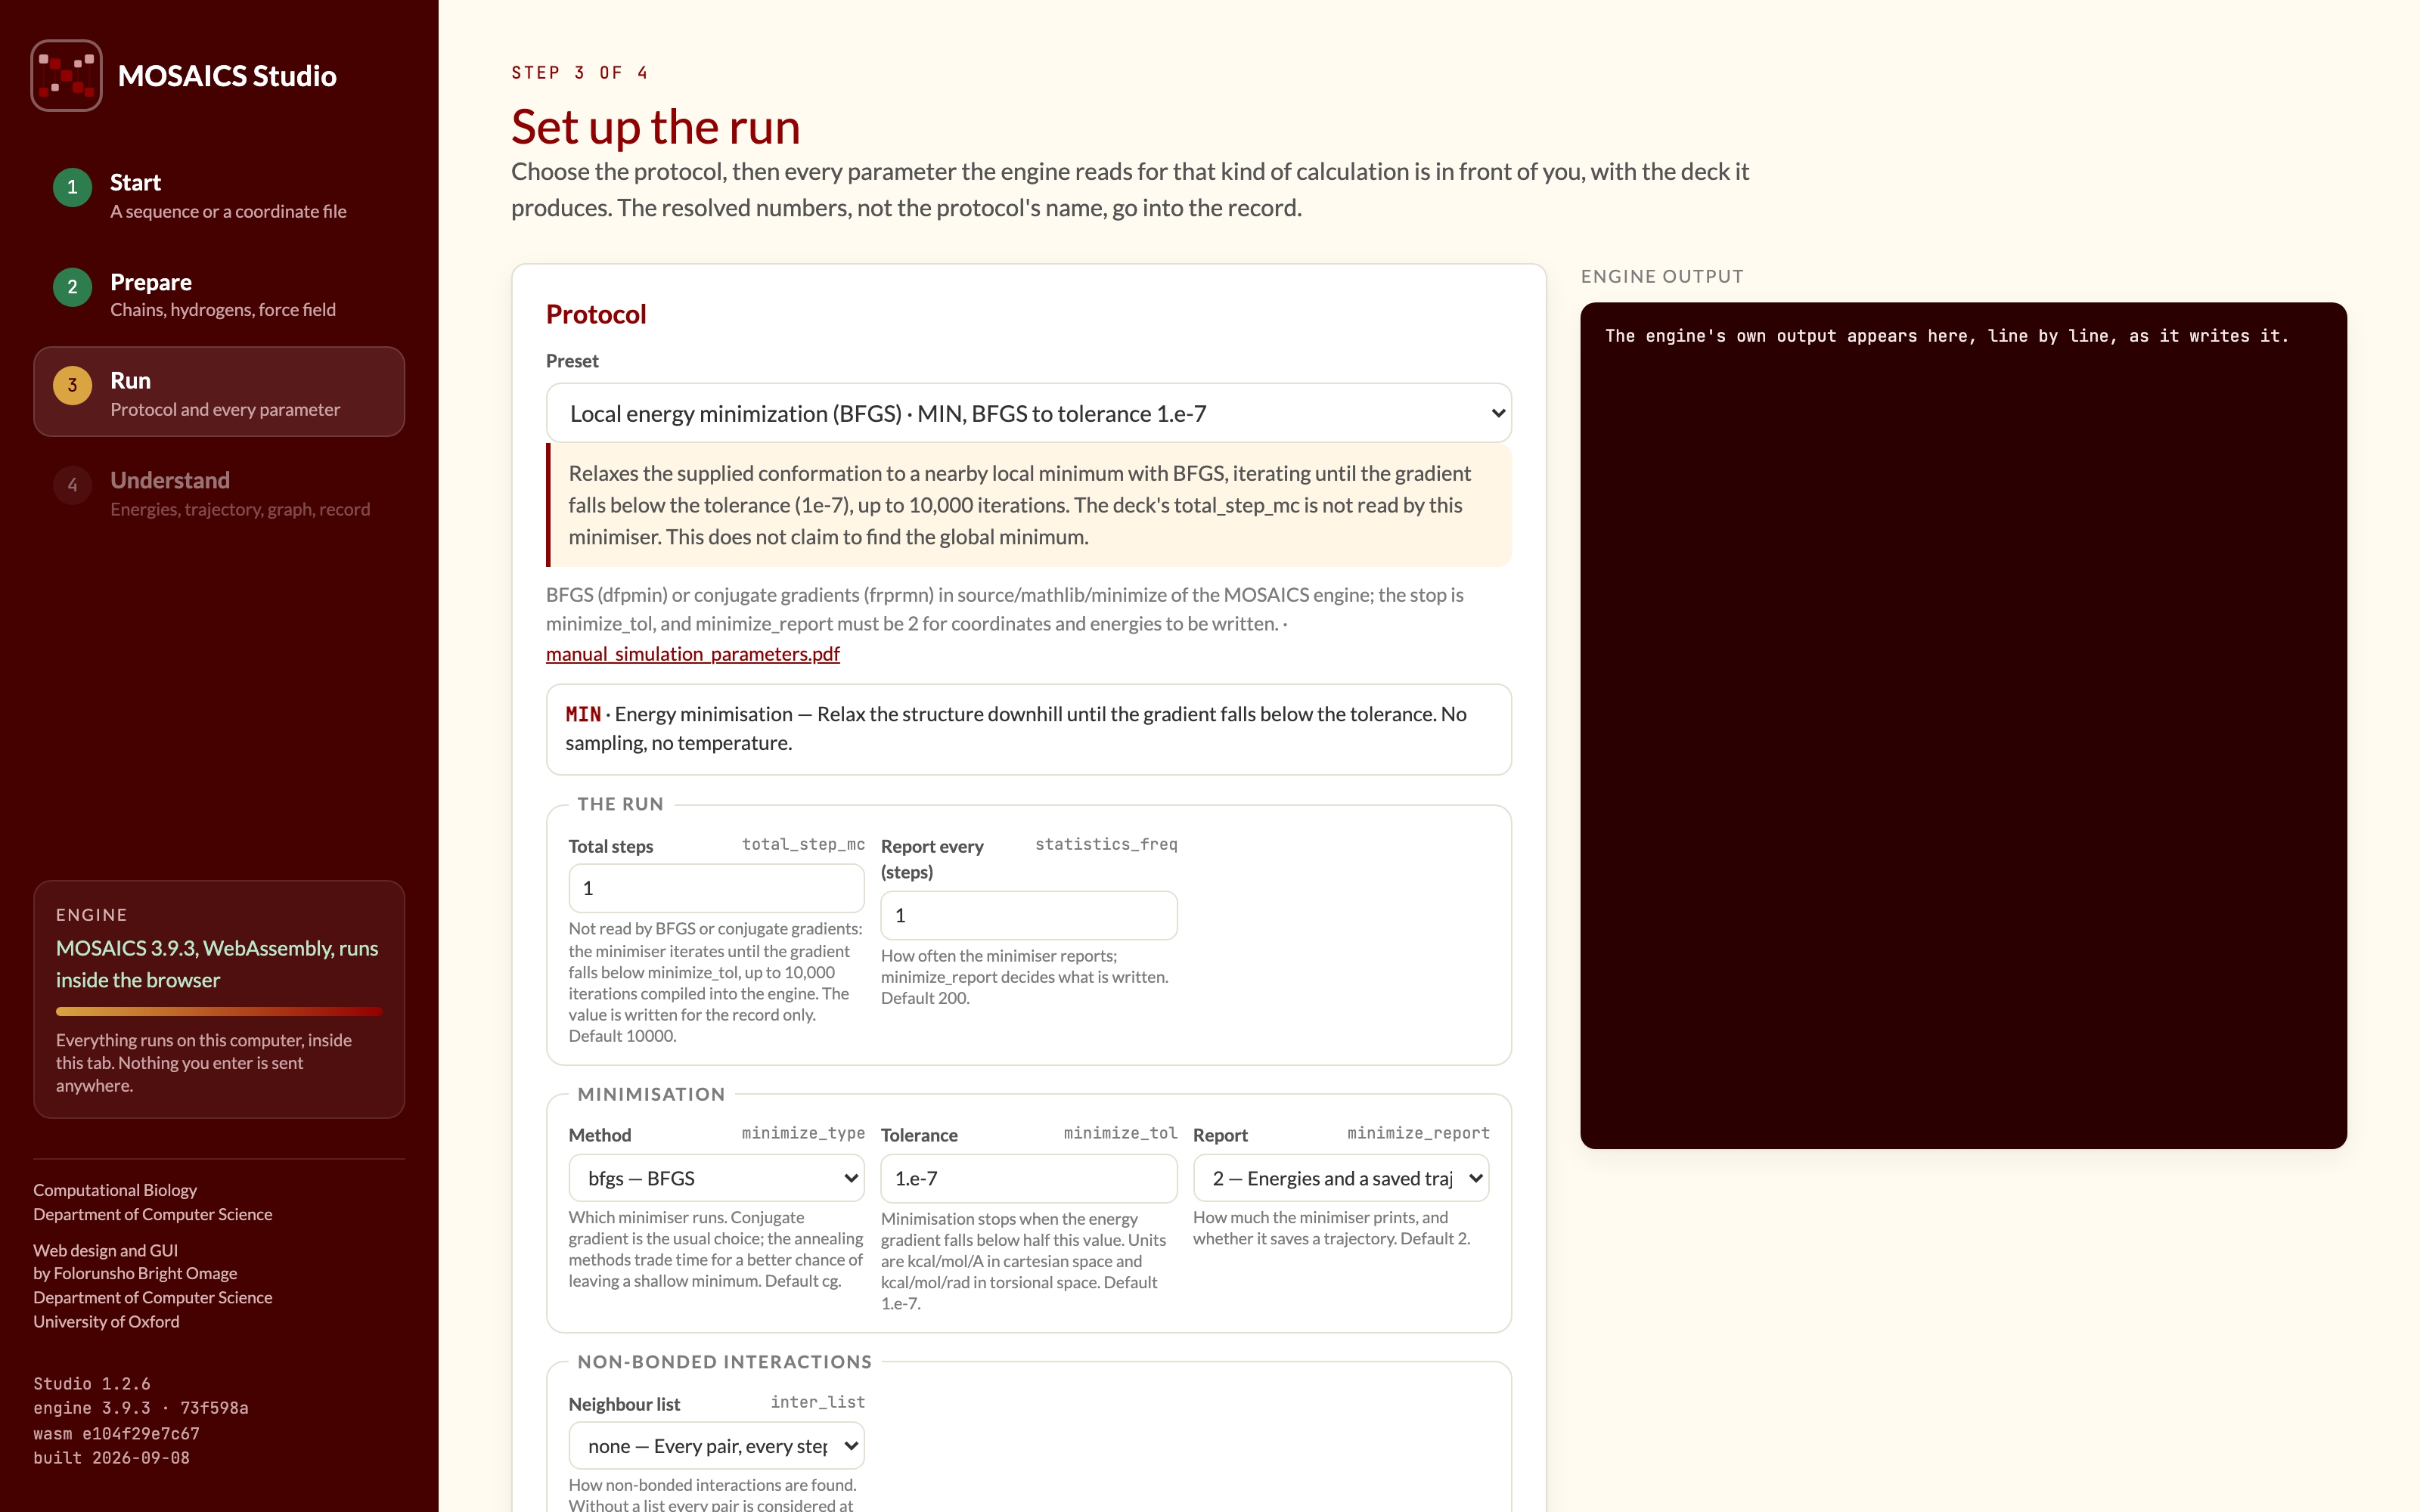
\includegraphics[width=\linewidth]{studio-run.png}
\caption{}
\end{subfigure}
\caption{\studio{} in the browser, version 1.2.6, the two steps not shown in
the main text. (a) Start: a sequence (DNA, RNA or a peptide), a topology and a
helical form, or a coordinate file; the default CGCGCG duplex is the one used
for the cross-check of Table~8 of the main text. (b) Run: the protocol chosen
from the fifteen the Studio offers, here the BFGS local minimisation with its
deck and its manual reference, and every parameter the engine reads for that
kind of calculation, grouped as the engine's manual groups them; the engine's
own output appears line by line in the right-hand panel as it runs.}
\end{figure}
\end{document}
